\section{moeo\-Entropy\-Metric$<$ Objective\-Vector $>$ Class Template Reference}
\label{classmoeoEntropyMetric}\index{moeoEntropyMetric@{moeoEntropyMetric}}
The entropy gives an idea of the diversity of a Pareto set relatively to another (Basseur, Seynhaeve, Talbi: 'Design of Multi-objective Evolutionary Algorithms: Application to the Flow-shop Scheduling Problem', in Proc.  


{\tt \#include $<$moeo\-Entropy\-Metric.h$>$}

Inheritance diagram for moeo\-Entropy\-Metric$<$ Objective\-Vector $>$::\begin{figure}[H]
\begin{center}
\leavevmode
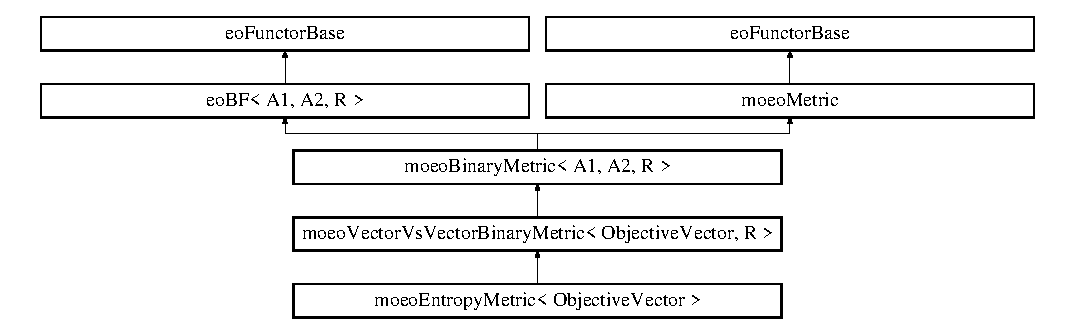
\includegraphics[height=4.03458cm]{classmoeoEntropyMetric}
\end{center}
\end{figure}
\subsection*{Public Member Functions}
\begin{CompactItemize}
\item 
double \bf{operator()} (const std::vector$<$ \bf{Objective\-Vector} $>$ \&\_\-set1, const std::vector$<$ \bf{Objective\-Vector} $>$ \&\_\-set2)
\begin{CompactList}\small\item\em Returns the entropy of the Pareto set '\_\-set1' relatively to the Pareto set '\_\-set2'. \item\end{CompactList}\end{CompactItemize}
\subsection*{Private Member Functions}
\begin{CompactItemize}
\item 
void \bf{remove\-Dominated} (std::vector$<$ \bf{Objective\-Vector} $>$ \&\_\-f)
\begin{CompactList}\small\item\em Removes the dominated individuals contained in \_\-f. \item\end{CompactList}\item 
void \bf{prenormalize} (const std::vector$<$ \bf{Objective\-Vector} $>$ \&\_\-f)
\begin{CompactList}\small\item\em Prenormalization. \item\end{CompactList}\item 
void \bf{normalize} (std::vector$<$ \bf{Objective\-Vector} $>$ \&\_\-f)
\begin{CompactList}\small\item\em Normalization. \item\end{CompactList}\item 
void \bf{compute\-Union} (const std::vector$<$ \bf{Objective\-Vector} $>$ \&\_\-f1, const std::vector$<$ \bf{Objective\-Vector} $>$ \&\_\-f2, std::vector$<$ \bf{Objective\-Vector} $>$ \&\_\-f)
\begin{CompactList}\small\item\em Computation of the union of \_\-f1 and \_\-f2 in \_\-f. \item\end{CompactList}\item 
unsigned int \bf{how\-Many\-In\-Niche\-Of} (const std::vector$<$ \bf{Objective\-Vector} $>$ \&\_\-f, const \bf{Objective\-Vector} \&\_\-s, unsigned int \_\-size)\label{classmoeoEntropyMetric_7977dac672bd6e2e1dfff8cf7954c180}

\begin{CompactList}\small\item\em How many in niche. \item\end{CompactList}\item 
double \bf{euclidian\-Distance} (const \bf{Objective\-Vector} \&\_\-set1, const \bf{Objective\-Vector} \&\_\-to, unsigned int \_\-deg=2)\label{classmoeoEntropyMetric_4716a673498a0681fb78414e390824a3}

\begin{CompactList}\small\item\em Euclidian distance. \item\end{CompactList}\end{CompactItemize}
\subsection*{Private Attributes}
\begin{CompactItemize}
\item 
std::vector$<$ double $>$ \bf{vect\_\-min\_\-val}\label{classmoeoEntropyMetric_e423d7d4416ef371ce7b0fd24c3212f8}

\begin{CompactList}\small\item\em vector of min values \item\end{CompactList}\item 
std::vector$<$ double $>$ \bf{vect\_\-max\_\-val}\label{classmoeoEntropyMetric_f5fad6d144520fd1403f774f98b18b99}

\begin{CompactList}\small\item\em vector of max values \item\end{CompactList}\item 
\bf{moeo\-Pareto\-Objective\-Vector\-Comparator}$<$ \bf{Objective\-Vector} $>$ \bf{pareto\-Comparator}\label{classmoeoEntropyMetric_227ce550253c35957300c6e11730c847}

\begin{CompactList}\small\item\em Functor to compare two objective vectors according to Pareto dominance relation. \item\end{CompactList}\end{CompactItemize}


\subsection{Detailed Description}
\subsubsection*{template$<$class Objective\-Vector$>$ class moeo\-Entropy\-Metric$<$ Objective\-Vector $>$}

The entropy gives an idea of the diversity of a Pareto set relatively to another (Basseur, Seynhaeve, Talbi: 'Design of Multi-objective Evolutionary Algorithms: Application to the Flow-shop Scheduling Problem', in Proc. 

of the 2002 Congress on Evolutionary Computation, IEEE Press, pp. 1155-1156) 



Definition at line 50 of file moeo\-Entropy\-Metric.h.

\subsection{Member Function Documentation}
\index{moeoEntropyMetric@{moeo\-Entropy\-Metric}!operator()@{operator()}}
\index{operator()@{operator()}!moeoEntropyMetric@{moeo\-Entropy\-Metric}}
\subsubsection{\setlength{\rightskip}{0pt plus 5cm}template$<$class Objective\-Vector$>$ double \bf{moeo\-Entropy\-Metric}$<$ \bf{Objective\-Vector} $>$::operator() (const std::vector$<$ \bf{Objective\-Vector} $>$ \& {\em \_\-set1}, const std::vector$<$ \bf{Objective\-Vector} $>$ \& {\em \_\-set2})\hspace{0.3cm}{\tt  [inline]}}\label{classmoeoEntropyMetric_191a8cdda7873e20338e678c5a7b927b}


Returns the entropy of the Pareto set '\_\-set1' relatively to the Pareto set '\_\-set2'. 

\begin{Desc}
\item[Parameters:]
\begin{description}
\item[{\em \_\-set1}]the first Pareto set \item[{\em \_\-set2}]the second Pareto set \end{description}
\end{Desc}


Definition at line 59 of file moeo\-Entropy\-Metric.h.

References moeo\-Entropy\-Metric$<$ Objective\-Vector $>$::compute\-Union(), moeo\-Entropy\-Metric$<$ Objective\-Vector $>$::how\-Many\-In\-Niche\-Of(), moeo\-Entropy\-Metric$<$ Objective\-Vector $>$::normalize(), moeo\-Entropy\-Metric$<$ Objective\-Vector $>$::prenormalize(), and moeo\-Entropy\-Metric$<$ Objective\-Vector $>$::remove\-Dominated().\index{moeoEntropyMetric@{moeo\-Entropy\-Metric}!removeDominated@{removeDominated}}
\index{removeDominated@{removeDominated}!moeoEntropyMetric@{moeo\-Entropy\-Metric}}
\subsubsection{\setlength{\rightskip}{0pt plus 5cm}template$<$class Objective\-Vector$>$ void \bf{moeo\-Entropy\-Metric}$<$ \bf{Objective\-Vector} $>$::remove\-Dominated (std::vector$<$ \bf{Objective\-Vector} $>$ \& {\em \_\-f})\hspace{0.3cm}{\tt  [inline, private]}}\label{classmoeoEntropyMetric_198a717fd0bab0bb91346399c1021f82}


Removes the dominated individuals contained in \_\-f. 

\begin{Desc}
\item[Parameters:]
\begin{description}
\item[{\em \_\-f}]a Pareto set \end{description}
\end{Desc}


Definition at line 113 of file moeo\-Entropy\-Metric.h.

References moeo\-Entropy\-Metric$<$ Objective\-Vector $>$::pareto\-Comparator.

Referenced by moeo\-Entropy\-Metric$<$ Objective\-Vector $>$::operator()().\index{moeoEntropyMetric@{moeo\-Entropy\-Metric}!prenormalize@{prenormalize}}
\index{prenormalize@{prenormalize}!moeoEntropyMetric@{moeo\-Entropy\-Metric}}
\subsubsection{\setlength{\rightskip}{0pt plus 5cm}template$<$class Objective\-Vector$>$ void \bf{moeo\-Entropy\-Metric}$<$ \bf{Objective\-Vector} $>$::prenormalize (const std::vector$<$ \bf{Objective\-Vector} $>$ \& {\em \_\-f})\hspace{0.3cm}{\tt  [inline, private]}}\label{classmoeoEntropyMetric_51dd04bdd0ac6315f4f5956fb726cec1}


Prenormalization. 

\begin{Desc}
\item[Parameters:]
\begin{description}
\item[{\em \_\-f}]a Pareto set \end{description}
\end{Desc}


Definition at line 138 of file moeo\-Entropy\-Metric.h.

References moeo\-Objective\-Vector$<$ Objective\-Vector\-Traits, double $>$::n\-Objectives(), moeo\-Entropy\-Metric$<$ Objective\-Vector $>$::vect\_\-max\_\-val, and moeo\-Entropy\-Metric$<$ Objective\-Vector $>$::vect\_\-min\_\-val.

Referenced by moeo\-Entropy\-Metric$<$ Objective\-Vector $>$::operator()().\index{moeoEntropyMetric@{moeo\-Entropy\-Metric}!normalize@{normalize}}
\index{normalize@{normalize}!moeoEntropyMetric@{moeo\-Entropy\-Metric}}
\subsubsection{\setlength{\rightskip}{0pt plus 5cm}template$<$class Objective\-Vector$>$ void \bf{moeo\-Entropy\-Metric}$<$ \bf{Objective\-Vector} $>$::normalize (std::vector$<$ \bf{Objective\-Vector} $>$ \& {\em \_\-f})\hspace{0.3cm}{\tt  [inline, private]}}\label{classmoeoEntropyMetric_2ed5771c3c611634b415f4be48cad172}


Normalization. 

\begin{Desc}
\item[Parameters:]
\begin{description}
\item[{\em \_\-f}]a Pareto set \end{description}
\end{Desc}


Definition at line 163 of file moeo\-Entropy\-Metric.h.

References moeo\-Objective\-Vector$<$ Objective\-Vector\-Traits, double $>$::n\-Objectives(), moeo\-Entropy\-Metric$<$ Objective\-Vector $>$::vect\_\-max\_\-val, and moeo\-Entropy\-Metric$<$ Objective\-Vector $>$::vect\_\-min\_\-val.

Referenced by moeo\-Entropy\-Metric$<$ Objective\-Vector $>$::operator()().\index{moeoEntropyMetric@{moeo\-Entropy\-Metric}!computeUnion@{computeUnion}}
\index{computeUnion@{computeUnion}!moeoEntropyMetric@{moeo\-Entropy\-Metric}}
\subsubsection{\setlength{\rightskip}{0pt plus 5cm}template$<$class Objective\-Vector$>$ void \bf{moeo\-Entropy\-Metric}$<$ \bf{Objective\-Vector} $>$::compute\-Union (const std::vector$<$ \bf{Objective\-Vector} $>$ \& {\em \_\-f1}, const std::vector$<$ \bf{Objective\-Vector} $>$ \& {\em \_\-f2}, std::vector$<$ \bf{Objective\-Vector} $>$ \& {\em \_\-f})\hspace{0.3cm}{\tt  [inline, private]}}\label{classmoeoEntropyMetric_4b99c1842d780a89bda08e99a59e3e29}


Computation of the union of \_\-f1 and \_\-f2 in \_\-f. 

\begin{Desc}
\item[Parameters:]
\begin{description}
\item[{\em \_\-f1}]the first Pareto set \item[{\em \_\-f2}]the second Pareto set \item[{\em \_\-f}]the final Pareto set \end{description}
\end{Desc}


Definition at line 177 of file moeo\-Entropy\-Metric.h.

Referenced by moeo\-Entropy\-Metric$<$ Objective\-Vector $>$::operator()().

The documentation for this class was generated from the following file:\begin{CompactItemize}
\item 
moeo\-Entropy\-Metric.h\end{CompactItemize}
